\documentclass[tikz,border=4pt]{standalone}
\usepackage{xcolor}
\definecolor{pdms}{HTML}{DCE5E8}
\definecolor{trace}{HTML}{8A6D25}
\definecolor{cell}{HTML}{34556E}
\begin{document}
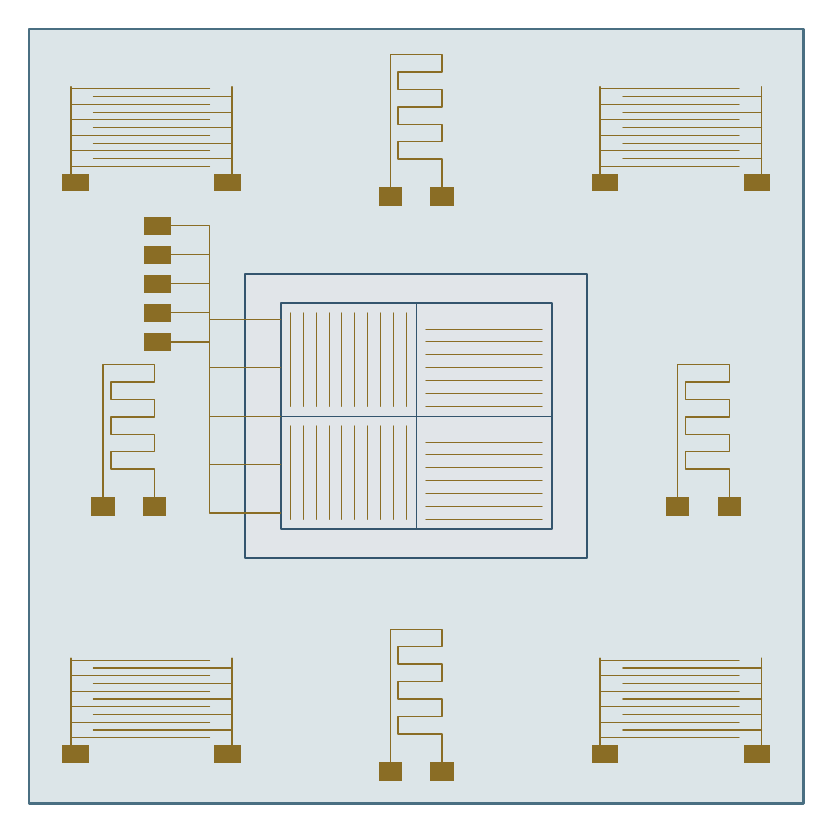
\begin{tikzpicture}[x=0.82cm,y=0.82cm,line cap=round,line join=round]
  % Nominal square slab.
  \fill[pdms] (0,0) rectangle (12,12);
  \draw[cyan!45!black,line width=0.8pt] (0,0) rectangle (12,12);

  % Humidity IDE: landscape footprint with alternating comb fingers.
  \newcommand{\humidity}[2]{%
    \begin{scope}[shift={(#1,#2)}]
      \draw[trace,line width=0.62pt] (0,0)--(0,1.35);
      \draw[trace,line width=0.62pt] (2.5,0)--(2.5,1.35);
      \foreach \y in {0.12,0.36,0.60,0.84,1.08,1.32}{
        \draw[trace,line width=0.40pt] (0,\y)--(2.15,\y);
      }
      \foreach \y in {0.24,0.48,0.72,0.96,1.20}{
        \draw[trace,line width=0.40pt] (0.35,\y)--(2.5,\y);
      }
      \fill[trace] (-0.13,-0.27) rectangle (0.28,0);
      \fill[trace] (2.22,-0.27) rectangle (2.63,0);
    \end{scope}}

  % Temperature meander: portrait footprint with one continuous serpentine.
  \newcommand{\temperature}[2]{%
    \begin{scope}[shift={(#1,#2)}]
      \draw[trace,line width=0.52pt]
        (0.20,0)--(0.20,2.05)--(1.00,2.05)--(1.00,1.78)--
        (0.32,1.78)--(0.32,1.51)--(1.00,1.51)--(1.00,1.24)--
        (0.32,1.24)--(0.32,0.97)--(1.00,0.97)--(1.00,0.70)--
        (0.32,0.70)--(0.32,0.43)--(1.00,0.43)--(1.00,0);
      \fill[trace] (0.02,-0.30) rectangle (0.38,0);
      \fill[trace] (0.82,-0.30) rectangle (1.18,0);
    \end{scope}}

  % Four corner humidity sensors from the supplied slab blueprint.
  \humidity{0.65}{9.75}
  \humidity{8.85}{9.75}
  \humidity{0.65}{0.90}
  \humidity{8.85}{0.90}

  % Four edge-centred temperature sensors from the supplied slab blueprint.
  \temperature{5.40}{9.55}
  \temperature{0.95}{4.75}
  \temperature{9.85}{4.75}
  \temperature{5.40}{0.65}

  % Central pressure/directional-shear sensor enclosure.
  \fill[cell!15] (3.35,3.80) rectangle (8.65,8.20);
  \draw[cell,line width=0.75pt] (3.35,3.80) rectangle (8.65,8.20);
  \draw[cell,line width=0.75pt] (3.90,4.25) rectangle (8.10,7.75);
  \draw[cell,line width=0.45pt] (6.00,4.25)--(6.00,7.75);
  \draw[cell,line width=0.45pt] (3.90,6.00)--(8.10,6.00);

  % Orthogonal dense electrode sectors.
  \foreach \x in {4.05,4.25,...,5.85}{
    \draw[trace,line width=0.32pt] (\x,6.15)--(\x,7.60);
    \draw[trace,line width=0.32pt] (\x,4.40)--(\x,5.85);
  }
  \foreach \y in {6.15,6.35,...,7.55}{
    \draw[trace,line width=0.32pt] (6.15,\y)--(7.95,\y);
  }
  \foreach \y in {4.40,4.60,...,5.80}{
    \draw[trace,line width=0.32pt] (6.15,\y)--(7.95,\y);
  }

  % Five-terminal routing concept, kept inside the slab.
  \foreach \y/\py in {7.50/8.95,6.75/8.50,6.00/8.05,5.25/7.60,4.50/7.15}{
    \draw[trace,line width=0.42pt] (3.90,\y)--(2.80,\y)--(2.80,\py)--(2.20,\py);
    \fill[trace] (1.78,\py-0.14) rectangle (2.20,\py+0.14);
  }
\end{tikzpicture}
\end{document}
